% mn2esample.tex
%
% v2.1 released 22nd May 2002 (G. Hutton)
%
%
% Previous versions of this sample document were
% compatible with the LaTeX 2.09 style file mn.sty
% v1.2 released 5th September 1994 (M. Reed)
% v1.1 released 18th July 1994
% v1.0 released 28th January 1994

\documentclass[useAMS,usenatbib]{mn2e}
\usepackage{graphicx}
%\usepackage{aas_macros}
\usepackage{multirow}
\usepackage{hyperref}


% If your system does not have the AMS fonts version 2.0 installed, then
% remove the useAMS option.
%
% useAMS allows you to obtain upright Greek characters.
% e.g. \umu, \upi etc.  See the section on "Upright Greek characters" in
% this guide for further information.
%
% If you are using AMS 2.0 fonts, bold math letters/symbols are available
% at a larger range of sizes for NFSS release 1 and 2 (using \boldmath or
% preferably \bmath).
%
% The usenatbib command allows the use of Patrick Daly's natbib.sty for
% cross-referencing.
%
% If you wish to typeset the paper in Times font (if you do not have the
% PostScript Type 1 Computer Modern fonts you will need to do this to get
% smoother fonts in a PDF file) then uncomment the next line
% \usepackage{Times}

%%%%% AUTHORS - PLACE YOUR OWN MACROS HERE %%%%%


%%%%%%%%%%%%%%%%%%%%%%%%%%%%%%%%%%%%%%%%%%%%%%%%

\title[Deconstructing M83]{Deconstructing a galaxy: identifying components of M83 with photometric clustering%
\footnote{  
Based on observations made with the NASA/ESA Hubble Space Telescope, obtained from the Data Archive at the Space Telescope Science Institute, which is operated by the Association of Universities for Research in Astronomy, Inc., under NASA contract NAS 5-26555. These observations are associated with program \#11360.
}
}
\author[Kiar \& Barmby \& Kiar]
{
P. Barmby$^{1}$\thanks{E-mail: pbarmby@uwo.ca} and 
A.K. Kiar$^{1}$\\
$^{1}$Department of Physics and Astronomy and Centre for Planetary Science and Exploration, University of Western Ontario, London, ON, N6A 3K7, Canada\\

}

\begin{document}

\date{}

%\pagerange{\pageref{firstpage}--\pageref{lastpage}} \pubyear{2002}

\maketitle
\label{firstpage}

\begin{abstract}
%\input{abs}
\end{abstract}

\begin{keywords}
keywords here
\end{keywords}

\section{Introduction}
Outline of intro:

\begin{enumerate}
\item Galaxies have a lot of discrete sub-components: stars, clusters, nebulae, nucleus.
\item One way to isolate specific components is with narrow-band filters or CMD analysis.
\item But what if you already have all the filters, and you want to make a census? Can start
with properties of known classes of objects \& pick out from multi-dimensional dataset.
\item Another approach is to see what blind clustering gets you: how many groups and what are they?
How does this depend on the (number of) wavelengths used?
\end{enumerate}

Work to be cited: 
\begin{itemize}
\item astro applications of k-means clustering 
\item astro applications of other ML techniques
\item general bkg on galaxy constituents
\item ??
\end{itemize}


\section{Data}
%\section{Data}

\subsection{Imaging dataset}
%\item intro to M83: global parameters (distance, size, environment)
The dataset used for this study is the Wide-Field Camera-3
Early Release Science (ERS) observations of the nearby spiral galaxy Messier 83 (M83).
M83 is a grand-design spiral of type SAB, located at a distance of 4.66~Mpc \citep{tully13}
and the largest member of the M83 subgroup of the nearby Centaurus group of galaxies \citep{tully15}.
The galaxy's apparent radius of $\sim12$~arcmin \citep{} is reasonably well-matched to the camera's field of view.
{\bf And here we note some other interesting things about M83.}

%\item Intro to WFC3 ERS dataset
%\item existing studies with this dataset (cluster, massive stars, etc)
% ref: chandar10, section. TODO: check for (unintentional!) plagiarism
The objective of the ERS observations as a whole was to probe star formation in galaxies.
The observations of M83 were made in broad- and narrow-band filters in order to characterize both stellar and nebular properties.
They cover a $3.6\times3.6$~kpc$^2$ region in the northern portion of the galaxy, including the nucleus,
a portion of a spiral arm and an interarm region.
The spatial resolution of the images is $0\farcs0396$~arcsec~pixel$^{-1}$,
corresponding to a linear scale of $XX$~pc~pixel$^{-1}$ at the 4.66~Mpc distance.
A complete description of the observations and data processing is given by \citet{chandar10};
our work here uses the observations in the UVIS channel, listed in Table~\ref{tab:filters}.
A number of previous studies have used the ERS M83 dataset for various purposes.
These include studies of 
star clusters \citep{chandar10, wofford11, whitmore11, bastian11, bastian12, fouesneau12, silva13, andrews14, chandar14, adamo15,ryon15,hollyhead15, sun16},
H~{\sc ii} regions \citep{liu13}, supernova remnants and the interstellar medium \citep{dopita10, hong11, blair14, blair15}, 
resolved stars \citep{kim12, williams15},
and a super-Eddington off-nuclear black hole \citep{soria14}.


\begin{table}
\centering
\caption{List of filters from ERS survey with band names and exposure times.}
\label{tab:filters}
\begin{tabular}{lll}
\hline\hline
Filter & Name & Exposure time\\
\hline
F225W &  Wide UV & 1800~s\\
F336W &  $U$-band & 1890~s\\ 
%F373N &  [\ion{O}{iii}] & 2400~s\\
F438W &  $B$-band & 1180~s\\
F487N &  H$\beta$ & 2700~s\\
%F502N &  [\ion{O}{ii}] & 2484~s
F555W &  V-band, South field & 1203~s\\
%F547M &  V-band, North field & \\
%F657N &  H$\alpha$+[\ion{N}{ii}]& 1484~s\\ 
%F673N &  [\ion{S}{ii}] & 1850~s\\
F814W &  $I$-band & 1203~s\\
\hline
\end{tabular}
\end{table}

We analyze the catalog produced by \citet{chandar10} and made available via **REF**, hereafter referred to as the `ERS catalog.'
The objects in this catalog were detected on a `white-light' image produced by a weighted combination of the $UBVI$ images.
Photometry in 0.5- and 3-pixel radius apertures at the positions of the detected sources was performed on the broad- and narrow-band images and tabulated in the Vega magnitude system. 
We apply the correction to the F657N magnitude zeropoint (from 20.72 to 22.35) noted in the header of the catalog.
\citet{chandar10} discussed aperture corrections for this catalog, but since we are primarily concerned with colours
and the aperture correction does not vary strongly with wavelength, we omit it.
The catalog contains about 68000 objects which are expected to include individual stars, star clusters, stellar blends,
supernova remnants, H${\sc ii}$ regions, planetary nebulae, and background galaxies.
%TODO: foreground stars?
Completeness and reliability of the catalog are not discussed by \citet{chandar10},
but a visual inspection of the the detected sources on the white-light image suggests that a reasonable balance
between completeness and reliability was achieved.
Nine objects are flagged in the catalog as being problematic 
and we remove them from our analysis.

As a check on the catalog we used Sextractor to detect and photometer objects in the individual images.
While the aperture photometry measurements matched well, the derived uncertainties were much smaller than those reported in the catalog.
Indeed, the catalog uncertainties seem to be physically unreasonable, with median uncertainty values well above 1~magnitude in
most bandpasses, and the catalog notes do not recommend them for use except in a relative sense.
Our comparison implied that recovering a more typical magnitude uncertainty distribution would be accomplished by
dividing the 0.5-pixel magnitude uncertainties  by 10 for the broad-band filters and 15 for the narrow-band filters.
This allows us to use the catalog aperture magnitudes as an indicator of detected signal-to-noise: our analysis uses only objects with
(scaled) 0.5-pixel magnitude uncertainties $<0.2$~mag.
For the remainder of the analysis we use magnitudes measured in the 0.5-pixel radius aperture, as these should be less affected
by crowding and the variable galaxy background.

Table~\ref{tab:cat_numbers} and Figure~\ref{fig:mag_unc} characterize the catalog in terms of measurements in individual filters.
Not all objects are detected in all filters;
Table~\ref{tab:cat_numbers} gives the number of objects for which photometry is reported in a given filter,
the number for which scaled 0.5-pixel magnitude uncertainty is $0.2$~mag or less,
and the aperture magnitude at which the median magnitude uncertainty is $0.2$~mag. % Discuss last column and why 555 - should be because it is the broad filter with the most detections used for the whitelight image?
Figure~\ref{fig:mag_unc} shows the distributions of magnitudes and uncertainties in a broad and narrow filter. % See appendix for complete list of figures

%AK: please calculate numbers here. For the last column scipy.stats.binned_statistic is a good way to do this.
%Numbers are calculated based on the 0.5 aperture filters - can be changed if we decide otherwise
\begin{table}
\centering
\caption{List of filter names with the number of objects detected, the number of objects with an uncertainty < 0.2 mag, and the 0.5 px aperture magnitude for which the median uncertainty is 0.2.}
\label{tab:cat_numbers}
\begin{tabular}{lrrlr}
\hline\hline
Filter & $N_{\rm obj}$ & $N_{\rm good}$ & $m_{\rm good}$ \\
\hline
F225W &  57237 & 15011 & m \\
F336W &  62192 & 34129 & m \\
F373N &  55966 & 8878 & m \\
F438W &  66356 & 48858 & m \\
F487N &  63812 & 13335 & m \\
F502N &  64313 & 14654 & m \\
F555W &  67424 & 65652 & m \\
F657N &  67782 & 67634 & m \\
F673N &  65305 & 25295 & m \\
F814W &  67050 & 59600 & m \\
\hline
\end{tabular}
\end{table}

%AK: here's where the plots go.
\begin{figure*}
\centering
\subfloat[Broad filter distribution.]{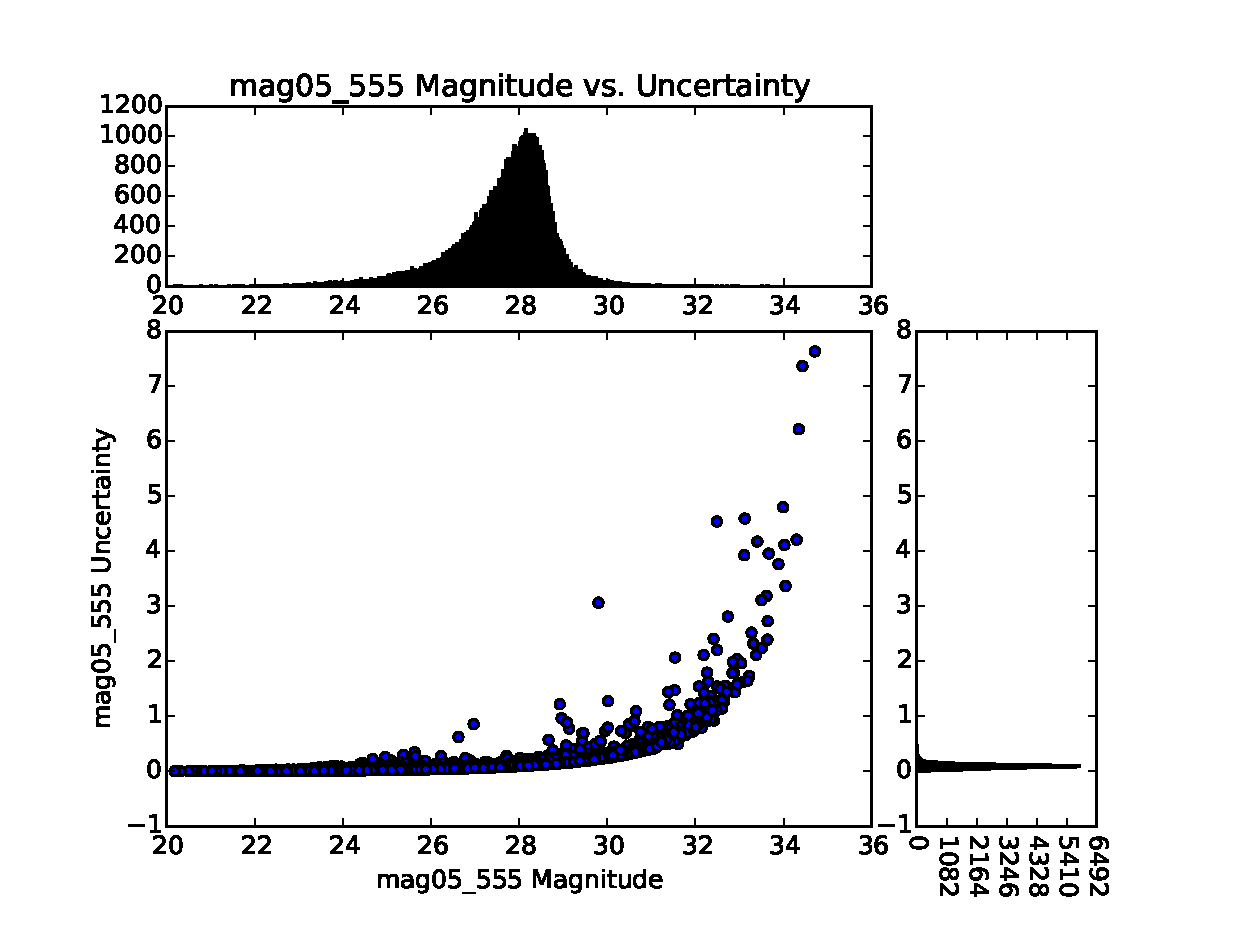
\includegraphics[width=0.5\textwidth]{figs/mag05_555_uncertainty_distribution}\label{fig:mag_unc_broad}}
\hfill
\subfloat[Narrow filter distribution.]{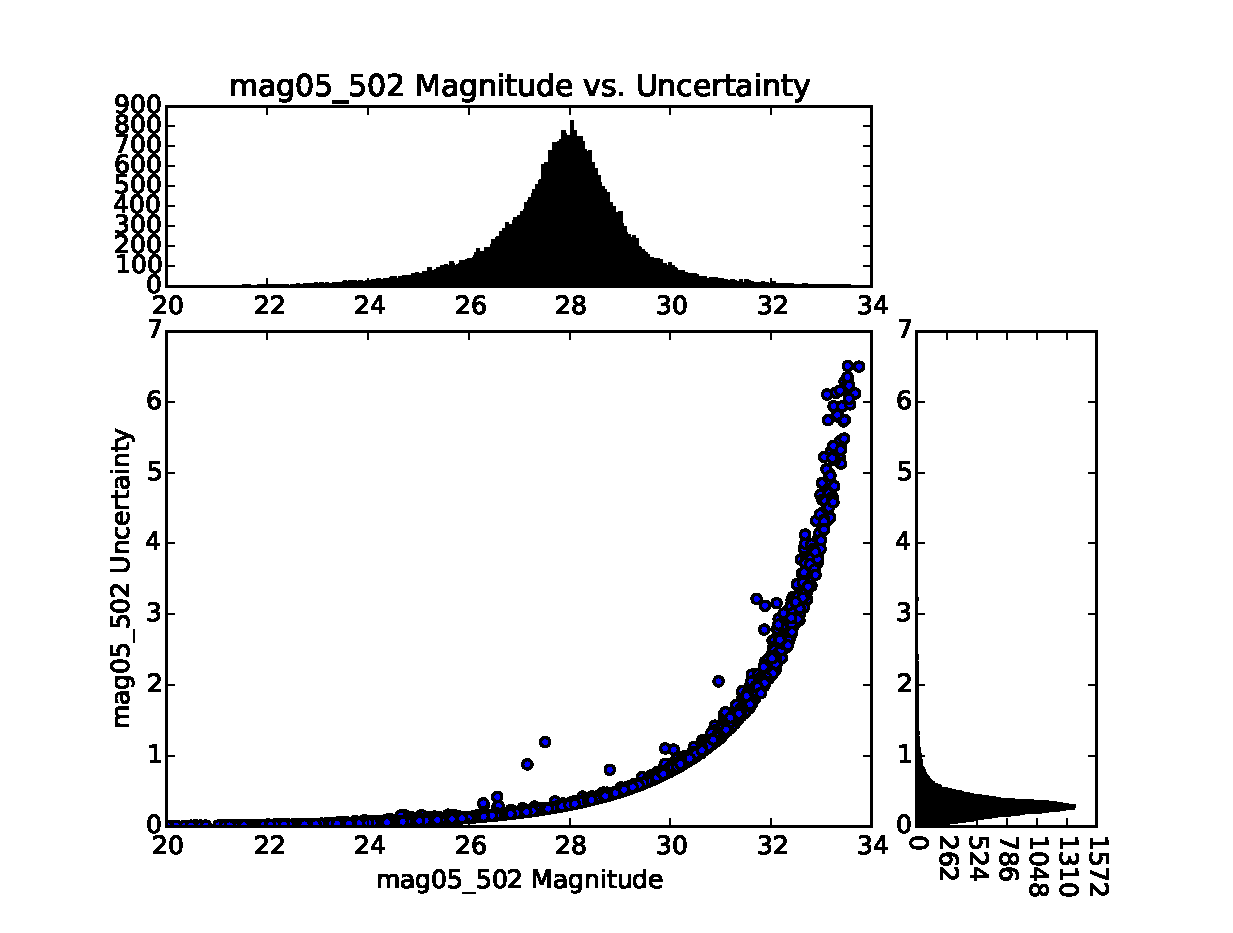
\includegraphics[width=0.5\textwidth]{figs/mag05_502_uncertainty_distribution}\label{fig:mag_unc_narrow}}
\caption{Distribution of magnitudes and uncertainties for objects in the \citet{chandar10} M83 ERS catalog.}
\label{fig:mag_unc}
\end{figure*}

\subsection{Colour Models}
\textbf{Discuss colour models. Figure is broad-band combination with model.}

\begin{figure}
\label{fig:model_colour}
\centering
\includegraphics[width=0.5\textwidth]{figs/data/plot_mag05_555-mag05_814vsmag05_336-mag05_438}
\caption{Colour-colour distribution of $V - I$ and $U - B$ with colour model plotted in pink.}
\end{figure}


\subsection{Published catalogs}

As one check on the results of our analysis, we use previously-published identifications of specific types of objects in M83.
We compiled a `published catalog' by combining the contents of the NASA Extragalactic Database (NED) and
[what does it stand for?] \citep[SIMBAD][]{wenger2000} and then adding the catalogs of Wolf-Rayet stars \citep{kim12} and
red supergiant candidates \citep{williams15}, which did not appear in either database.
NED's focus as an extragalactic database and SIMBAD's focus on Galactic objects mean that their contents overlap but are not identical, 
and this is true of the area surrounding M83. A $3\farcm3$ radius region around the coordinates centered at  ($204.26761\deg, -29.839939\deg$)
contains 1553 NED objects and 1772 SIMBAD objects, of which 1220 are matched with each other at 1\arcsec tolerance.
Although the two services use slightly different naming conventions, with human inspection the matches are generally recognizable as referring
to the same object. Interestingly, the databases do not always report the same object type even when the names are identical.
The differences are reasonable in some cases (a supernova remnant can also be an X--ray source, for example), but not others
(e.g. CXOU J133703.0-294945 is reported as a supernova remnant by SIMBAD and an H${\sc ii}$  region by NED).
A detailed study of the databases is beyond the scope of this work; for the purposes of this analysis, we kept the NED classification
for objects which appeared in both databases.
Objects which appeared in one database but not the other were primarily from recent work \citep[e.g.][]{long2014}, from
older studies likely superseded by newer ones \citep[e.g.][]{larsen1999}, or from studies in which only coordinates relative to
the galaxy centre were given \citep{rumstay83,dvpd83}.

Our final combined catalog has 2425 objects of which 750**check** are in the region covered by the ERS catalog.
The main classes are star clusters (350), X--ray sources (105), supernova remnants (86), H${\sc ii}$ regions (81),  and
radio sources (36).
Nearly every entry in the published catalog had an ERS catalog object within 1\arcsec, and the mean distance between
matched objects was 0\farcs26.
Given the nearly 100-fold difference in object density between the two catalogs, matching based on positions alone may 
result in spurious matches **REF**. *Some discussion of the exact matching procedure is warranted here, and a conclusion
on what the best thing to do is.**


%Outline for data section
%%\begin{enumerate}
%\item Intro to WFC3 ERS dataset
%\item intro to M83: global parameters (distance, size, environment)
%\item existing studies with this dataset (cluster, massive stars, etc)
%\item description of catalog (is there a ref for this??)
%\item anything about these data we don't like/didn't use?

%\end{enumerate}



\section{Analysis}
% Analysis section
This section will outline colour construction, the clustering process, and the selection of the optimal clustering for each colour combination.
Each colour combination was clustered using the same process, and in two and three dimensions.

\subsection{Colour Selection}

Observations in 10 bands allow the generation of 45 different colours, but not all of these colours are likely to be useful in characterizing components of the galaxy.
Since the average survey consists of four filters, different combinations of four filters were used to construct colours for clustering. 
Due to the large number of filters available in the ERS data, the combinations had to be narrowed down to a reasonable set.
Two types of colour combinations were created: combinations of all broad band filters, and combinations with one narrow band and three broad bands.
Additionally, two and three dimensions were considered for clustering, in order to maximize the use of the data in an average survey.

\subsubsection{Broad Band Combinations}

\textbf{PB: Should we explain what kind of objects we hope to find in these combos?}

The first type of combination was comprised of the broad band filters: F336W (U), F438W(B), F555W(V), and F814W(I).
The F225W (UVW) filter was not included in this set as it is not a standard filter most surveys.
Additionally, the $U - I$ colour was not used in the analysis because it was determined that this colour was not physically meaningful.
This is because it is unlikely that an object would emit a detectable reading in both these bands due to their distance from one another in wavelength.
Using the four filters, the broad band colour combinations created can be found in Table~\ref{tab:BBcolours}.
These combinations were created in order to remove any obvious correlation between the colours that could occur by the inclusion of the same band in both colours.

\begin{table*}
\centering
\caption{Broad band colour combinations and the number of objects detected in each colour, and in each combination, with uncertainties less than $0.2$.}
\label{tab:BBcolours}
\begin{tabular}{lllllll}
\hline\hline
Colour 1 & Objects & Mean Uncertainty & Colour 2 & Objects & Mean Uncertainty & Combined Objects \\
\hline
$U - B$ &  33523 & 0.1606 mag & $V - I$ &  57935 & 0.1334 mag & 28931\\
$U - V$ &  33692 & 0.1429 mag & $B - I$ &  41413 & 0.1590 mag & 28931\\
$B - V$ &  48660 & 0.1456 mag & $ - $ & $ - $ & $ - $ & $ - $ \\
\hline
\end{tabular}
\end{table*}

\subsubsection{Narrow Band Combinations}

\textbf{PB: Should we explain more about why we choose to do Broad - Narrow? And what objects we hope to find in these combos?}

The second set of combinations included the narrow band filters: F373N ($O_{2}$), F487N ($H\beta$), F502N ($O_{3}$), F657N ($H\alpha$), and F673N ($S_{2}$).
In addition, the broad band F225W (UVW) was included in this set to ensure its data was included in the analysis. 
Colours were created with the narrow bands by pairing them with the broad bands that covered them in wavelength space.
These colours were created in order to reduce the number of possible combinations that could be used for analysis.
The second colour in each combination was created from two broad bands that did not overlap the first colour in wavelength space.
Table~\ref{tab:NBcolourcombos} lists the narrow band colour combinations used for analysis.
The number of objects in the narrow band combination, with the exception of the $H\alpha$ band, is significantly lower than the broad band combinations.
These combinations were useful for analysis as their distributions were not as dense as the broad bands, and the clustering algorithms were able to detect interesting structure within them.
Making colours out of a combination of broad and narrow bands ensure that the objects clustered in these bands are physically meaningful, as it is likely that the object would emit in the broad band that contains the narrow band. \textbf{Not sure if that is a reason why we chose to construct them that way}.

\begin{table*}
\centering
\caption{Narrow band colour combinations and the number of objects detected in each colour, and in each combination, with uncertainties less than $0.2$.}
\label{tab:BBcolours}
\begin{tabular}{lllllll}
\hline\hline
$Narrow - Broad$ & Objects & Mean Uncertainty & $Broad - Broad$ & Objects & Mean Uncertainty & Combined Objects \\
\hline
$UVW - U$ &  14977 & 0.1539 mag & $B - V$ &  48660 & 0.1456 mag & 14943 \\
$ - $ & $ - $ & $ - $ & $B - I$ &  41413 & 0.1590 mag & 14095 \\
$ - $ & $ - $ & $ - $ & $V - I$ &  57935 & 0.1334 mag & 14098 \\
\hline
$U - O_{2}$ & 8675 & 0.1504 mag & $B - V$ &  48660 & 0.1456 mag & 8657 \\
$ - $ & $ - $ & $ - $ & $B - I$ &  41413 & 0.1590 mag & 8558 \\
$ - $ & $ - $ & $ - $ & $V - I$ &  57935 & 0.1334 mag & 8559 \\
\hline
$B - H\beta$ & 13269 & 0.1493 mag & $V - I$ &  57935 & 0.1334 mag & 13147 \\
\hline
$O_{3} - V$ & 14644 & 0.1418 mag & $U - B$ &  33523 & 0.1606 mag & 13390 \\
\hline
$H\alpha - I$ & 59465 & 0.1495 mag & $U - B$ &  33523 & 0.1606 mag & 28920 \\
$ - $ & $ - $ & $ - $ & $U - V$ &  33692 & 0.1429 mag & 29060 \\
$ - $ & $ - $ & $ - $ & $B - V$ &  48660 & 0.1456 mag & 41317 \\
\hline
$S_{2} - I$ & 25185 & 0.1535 mag & $U - B$ &  33523 & 0.1606 mag & 14577 \\
$ - $ & $ - $ & $ - $ & $U - V$ &  33692 & 0.1429 mag & 14586 \\
$ - $ & $ - $ & $ - $ & $B - V$ &  48660 & 0.1456 mag & 18882 \\
\hline
\end{tabular}
\end{table*}

\subsubsection{Number of Dimensions}
Due to the high number of bands available in the ERS data, the number of dimensions available to cluster was very high.
Limiting the number of band combinations through the system outlined above helped reduce the number of dimensions.
However, in addition to the two dimensional combinations, clustering in three dimensions was investigated.
Three dimensional colour combinations were created based on the combinations listed in Table~\ref{tab:BBcolours} and Table~\ref{tab:NBcolourcombos}.
In the broad band combinations, three dimensional colour spaces were created by making colours with a common band, either B or V.
These bands were selected in order to avoid creating the $U - I$ colour.
\textbf{PB: Not sure if this next sentance explains why we chose to use a common band clearly. Just trying to say that the colours could be subtracted to transform back into the two dimensional space.}
A common band was used in all colours in order to create a three dimensional space that of colours that could be transformed back into the original two dimensional space. 

In the narrow band combinations, the three dimensional colour spaces were created by making colours with the narrow band common between them.
Similar to the broad band spaces, these combinations could be transformed into the original two dimensional space, and act as an extension of the two dimensional distribution.

Clustering in three dimensions increased the complexity of the distribution, creating more information for the clustering algorithms to use.
However, limiting the dimensionality of the problem to three allowed the analysis to stay within the constraints of a common survey.
A space of up to 45 dimensions could have been created, but that space would not be reasonable for the analysis of a common survey.

\subsection{Clustering Process}
Clustering was performed using all methods for each colour combination. 
The following process allowed the investigation of the effect of all paramters on each clustering technique, leading to the selection of an optimal clustering.

\subsubsection{Meanshift}
Mean-Shift clustering was performed first by estimating the bandwidth paramter with the $estimate-bandwidth$ function in $scikit-learn$. \textbf{How do we cite this package?}
This function estimates the bandwidth parameter based on the distances between points in the dataset, and determines if the distribution has high or low variance.
Following the initial clustering, a the bandwidth was varried and the clustering was performed again with bandwidth values on intervals of $\pm 0.1$ from the estimated bandwidth value.
Varying the bandwidth revealed how sensitive a combination was to the parameter.
If a combination was very sensitive to bandwidth, then the number of clusters that meanshift would predict would vary greatly over a small range of bandwidth values.
This type of combination usually resulted in poor segmentation, as the algorithm would not converge on a number of clusters. 
However, sensitivity could also be the result of the starting bandwidth estimate.
If the original estimate was in an unstable bandwidth interval, then the hierarchy would reflect that, and the testing of multiple bandwidth values could result in convergence.

\subsubsection{Affinity Propagation}
Affinity Propagation clustering was performed after Meanshift. 
The first clustering was run using the preference estimations outlined in Section 3. \textbf{how to referene section}.
The preferences were set to the median and the minimum value of the similarities, and the damping factor was kept at the default value of $0.5$.
This resulted in a segmentation with over 100 clusters in multiple colour combinations.
The preferences were then set to 10\% of the number of objects in the data set, and the damping factor was set at $0.95$.
With these parameters, the clusterings varried significantly over differnet colours. 
The clusterings were repeated to try and reveal a trend in the parameters, but the algorithm was too sensitive for this size of dataset.
Following the initial tests of Affinity Propagation, it was determined that this clustering method was not effective.
Due to the number of computations required for the calculation of the messages passed between points on each iteration, the algorithm was very sensitive to the input parameters, and did not produce meaningful clusterings.
The algorithm is effective for small and medium sized datasets, and was able to create some reasonable clusters when the uncertainty limit was set at $0.1 mag$, which reduced the number of objects significantly. 
After multiple clusterings, a systematic way of determine the correct number of clusters could not be determined, and the algorithm was not used further.

\subsubsection{K-Means}
K-Means clustering was performed last.
The first clustering was performed using the number of clusters determined from the initial clusterings by Meanshift.
Next, K-Means was performed with $K = \pm 4$ from the original clustering.
This method of clustering was similar to the Meanshift approach, as it revealed how the dataset reacted to different values of $K$.
K-Means was the most efficient algorithm of the three, as it produced clusterings quickly, and always produced clusters of reasonable size.

\subsection{Selecting the Optimal Clustering}
Determining the optimal clustering was the most difficult task of the analysis.
Selecting the optimal clustering can often seem arbitrary, as no ``right" answer is obvious.
In order to determine the optimal clustering, a variety of metrics and statistics were calculated to evaluate each cluster.
Additionally, the relationships between a variety of clustering parameters were investigated to try and determine where they indicated the optimal clustering.
Since the performance of the algorithms was directly related to the parameters used as input, those relationships were critical for selecting the clustering.
The objects in each cluster were then found in the white-light image of M83, to determine if there was a relationship between the objects assigned to the same cluster and their spatial position.
Finally, colour models were created and imposed on the cluster distribution to determine if the segmentation agreed with a model. \textbf{Need more on why the models were used}.

\subsubsection{Silhouette Score}
The silhouette score is a metric used to describe the compactness of a cluster in a given clustering and is calculated as an average of all samples in a clustering.  
The silhouette score is given by:

\begin{equation}
\label{eq:ss}
Silhouette Score = \frac{b - a}{\textit{max}\big(a, b\big)}
\end{equation}

where $a$ is the mean intra-cluster distance, and $b$ is the distance between a point and the nearest cluster that point is not a member of.
The score was used in two ways.
First, the average score was calculated for a given clustering.
This calculated the average score across all data in the sample.
Next, the average score for each cluster was computed.
The average cluster score evaluates the strength of a given cluster within a clustering.
This metric allowed each cluster to be evaluated individually, and revealed which clusters were responsible for the average score of the clustering.
Additionally, the average score allowed seemingly arbitrary clusters to be evaluated.
If the segmentation did not seem meaningful, the average score would reveal if the cluster was isolated and compact.
This revealed the significance of clusters that could have been viewed as noise or outliers. \textbf{This section needs more explaination}.

\textbf{Struggling to explain why that is how the score works}. 
Ideally, the silhouette score for the entire clustering should peak near the center of the distribution indicating the optimal clustering. 
High scores where the number of clusters is low often do not reflect the structure of the distribution, while high numbers of clusters are often imposed on the data as a result of the specified parameters.
This is often not the case, as seen in Figure~\ref{fig:sscore}, which shows the distribution of the silhouette score against the number of clusters.
For the K-Means clusterings, the score does not peak in the center of the distribution.
Instead of selecting the clustering with the highest score, the optimal clustering is found where the relation begins to elbow; between 4 and 5 clusters.
This clustering is selected because any increase in $K$ after this point does not affect the score, and does strengthen or weaken the clustering.
This means that the algorithm has found the balance between the natural clusters in the distribution and artificially segmenting the data.

\begin{figure}[H]
\centering
\includegraphics[width=\linewidth]{figs/methods/silhouette_score_relation}
\caption{Distribution of the silhouette score as a result of the number of clusters imposed for the $UVW - U$ and $V - I$ colours. The \textit{blue} points are the scores of Meanshift clustering, \textit{red} points are scores of K-Means.}
\label{fig:sscore}
\end{figure}

The distribution of score as a result of the Meanshift algorithm does not follow the same pattern.
The silhouette score was not as successful at describing the strength of Meanshift clusterings as Meanshift often created one large cluster and several smaller ones, which is not considered strong by the score.
In order to determine the optimal Meanshift clustering, other relationships were investigated.

\subsubsection{Cluster Statistics}
Various statistics were calculated to help describe the similarity between the objects in a given cluster.
The standard deviation and average colour was calculated for each colour, and each cluster within a clustering. 
These metrics helped describe the distribution of the objects in the colour-colour space within a cluster. 
Clusters that had large standard deviations were viewed as too dissimilar to be a meaningful cluster, and clusters whose averages varried significantly from the cluster centers were disgarded.

\textbf{I'm not sure that this paragraph describes why we calculated the fractional size}.
The fractional size of each cluster was also calculated and described the distribution of objects between clusters.
If a clustering segmented the objects into a large cluster followed by several smaller ones, the clustering was investigated further, as this segmentation could mean one of two things. 
This type of clustering could be a result of the identification of interesting objects, in which case the clustering algorithm was able to identify the objects and place them in the same cluster.
However, this type of clustering could also be a result of the underlying distribution of the data, as the clustering techniques are largely drawn to areas of high density.
If this is the case, the clustering only created the smaller clusters as a result of the parameters imposed on the clustering.

\subsubsection{Parameter Relationships}
In addition to metrics, the relationships between various parameters were investigated to determine how the each clustering method behaved.

Each K-Means clustering was checked by plotting the sum-of-squares value for each value of $K$.
Figure~\ref{fig:inertia} shows the inertia distribution for the $H\beta - B$ vs. $V - I$ colour.
As $K$ increases, the inertia value decreases as the inertia value represent the total distance between the total distance between the points of each cluster.
The value decreases with $K$ as the total distance in each cluster decreases as more clusters are introduced.
This distribution was used to check the clustering and ensure that the clusterings were successful.

\begin{figure}[H]
\centering
\includegraphics[width=\linewidth]{figs/methods/inertia_plot}
\caption{Distribution of the inertia as a result of the number of clusters for the $H\beta - B$ and $V - I$ combination.}
\label{fig:inertia}
\end{figure}

Following the inertia test, the cluster centers were tested by running K-Means for 40 trials with the same value of $K$.
This test was run to determine if the clusterings were stable as K-Means is initiallized randomly, and the clusters produced can depend on the starting position.
Figure~\ref{fig:cen_test} shows the result of the three dimensional clustering test for the $U - O_{2}$ and $B - V$ combination.

\begin{figure}[H]
\centering
\includegraphics[width=\linewidth]{figs/methods/3_cl_cluster_centers}
\caption{Distribution of the cluster center as a function of the trial number for the three dimensional $U - O_{2}$ and $B - V$ combination with $K=3$. The left panel plots the centers in the $U - O_{2}$ colour, and the right panel plots the centers in the $B - V$ colour. Each line of dots represents a single cluster, and the colours represent the cluster number.}
\label{fig:inertia}
\end{figure}

It is clear that each initialization found different clusters first as the colours in each line are not constant. 
Despite the random initialization the final cluster centers did not change.
This distribution of cluster centers represents a strong clustering. 
If the cluster centers vary across multiple initializations of K-Means, the clustering would not be reliable, and the combination would not be considered for analysis.

The behavior of the bandwidth parameter was investigated for each Meanshift clustering.
Figure~\ref{fig:bad_ms} shows the relation between the score and number of clusters for the three dimensional $U - O_{2}$ and $B - I$ combination.
The blue dots represent the Meanshift clusterings.

\begin{figure}[H]
\centering
\includegraphics[width=\linewidth]{figs/methods/silhouette_score_bad_ms}
\caption{Distribution of the silhouette score as a result of the number of clusters imposed for the three dimensional $U - O_{2}$ and $B - I$ combination. The \textit{blue} points are the scores of Meanshift clustering, \textit{red} points are scores of K-Means.}
\label{fig:bad_ms}
\end{figure}

It is clear that an optimal clustering cannot be determined from this relation, as the score decreases linearly with the number of clusters Meanshift predicts.
The Mean-Shift scores do not follow a similar distribution as K-Means, as the accuracy of Meanshift is related to the bandwidth parameter, seen in Figure~\ref{fig:bwscore}.
The optimal Mean-Shift clustering was chosen by finding the bandwidth where the relation between the bandwidth and number of clusters reached an elbow, or where the relation between bandwidth and silhouette score elbowed.
In both panels of Figure~\ref{fig:bwscore} that the bandwidth parameter predicts five clusters.
Both distributions elbow at the same bandwidth interval, maximizing the score and predicting the same number of clusters for bandwidth valeus following the elbow.
The bandwidth parameter was the primary indicator of the optimal Meanshift clustering.
If a trend could not be found with the bandwidth parameter, then the silhouette score and number of clusters was investigated.

\begin{figure}[H]
\centering
\includegraphics[width=\linewidth]{figs/methods/meanshift_parameters}
\caption{Distribution of the silhouette score as a function of bandwidth, and the distribution of the number of clusters as a function of bandwidth.}
\label{fig:bwscore}
\end{figure}

\section{Results}
% Results section

\[ To be reorganized \]

The results of the analysis are grouped into the type of band used to make each colour.  % More general notes about results

\subsection{Broad \& Broad Band Combinations}

\subsection{Broad \& Narrow Band Combinations}
Each broad and narrow band combination was tested against every broad-broad band combination that did not boarder the narrow band.

\subsubsection{UVW - U}
The UVW - U combination was tested clustered with the B-I, V-I, and B-V colours. % More general information about what we are looking for in this combination

\paragraph{Mean-Shift}
When clustered using Mean-Shift, a similar pattern of clustering was seen in all combinations.
Due to the structure of the Mean-Shift algorithm, it is drawn towards areas of high density in the distribution. % Refernce meanshift paper
Since the distribution of the UVW-U combinations were generally consentrated around zero in the colour-colour space, the Mean-Shift algorithm would pick out one large cluster with many smaller ones. 
Each smaller cluster had to be investigated to determine if the algorithm had found a meaningful cluster, or if it had just clustered noise.
In order to determine this, a cluster hierarchy was created with different bandwidth values to see how long each cluster lasted in the bandwidth space. 
If a small cluster was created at a low bandwidth level and stayed alive until the number of clusters became 2-3, then it is reasonable to assume that the cluster was meaningful.
Figure ~\ref{fig:UVWMS1} shows the result of one trial of Mean-Shift clustering with $h=0.6$ which created 4 clusters. 
Figure ~\ref{fig:UVWMS2} shows the result of one trial of Mean-Shift clustering with $h=0.4$, creating 10 clusters. 
The structure of cluster $2$ in both Figure ~ref{fig:UVWMS1} and Figure ~ref{fig:UVWMS2} can be seen distinctly. 
This cluster would have been viewed as noise if the hierarchy was not created, but after testing multiple bandwidth values, it can be seen that these objects are significant. 

\begin{figure}[H]
\centering
\includegraphics[width=\linewidth]{figs/meanshift_color_4cl_mag05_225-mag05_336vsmag05_555-mag05_814}
\caption{Colour-Colour distribution of the UVW-U and V-I colours, clustered using Mean-Shift with $h=0.6$. The colour of each point corresponds to the cluster the point was assigned to. Cluster numbers can be seen in the legend.}
\label{fig:UVWMS1}
\end{figure}

\begin{figure}[H]
\centering
\includegraphics[width=\linewidth]{figs/meanshift_color_10cl_mag05_225-mag05_336vsmag05_555-mag05_814}
\caption{Colour-Colour distribution of the UVW-U and B-I colours, clustered using K-Means with $h=0.4$. The colour of each point corresponds to the cluster the point was assigned to. Cluster numbers can be seen in the legend.}
\label{fig:UVWMS2}
\end{figure}

\paragraph{K-Means}

When clustered using K-Means, two types of results were seen.
Figure ~\ref{fig:UVWKM1}, shows the result of K-Means clustering for $K=5$ against the B-V colour. 
\begin{figure}[H]
\centering
\includegraphics[width=\linewidth]{figs/kmeans_xy_5cl_mag05_225-mag05_336vsmag05_438-mag05_555}
\caption{Colour-Colour distribution of the UVW-U and B-V colours, clustered using K-Means with $K=5$. The colour of each point corresponds to the cluster the point was assigned to. Cluster numbers can be seen in the legend.}
\label{fig:UVWKM1}
\end{figure}
The algorithm split the data into groups based on its UVW - U colour. The pattern continued for all values of K, and the S Scores of the combination elbowed at $K=5$.
The second type of result for K-Means can be seen in Figure ~\ref{fig:UVWKM2}, against the B-I colour. 
This clustering segmented the data into circular groups within the distribution. 
Similar to the B-V combination, the S Score elbowed at $K=5$. 
When the objects were plotted on the whitelight image, both types of segmentation seemed to pick out objects that live in different structures of M83. % Reference Chandar
% Add test with CLAsPS score to show correlation with labels 
\begin{figure}[H]
\centering
\includegraphics[width=\linewidth]{figs/kmeans_xy_5cl_mag05_225-mag05_336vsmag05_438-mag05_814}
\caption{Colour-Colour distribution of the UVW-U and B-I colours, clustered using K-Means with $K=5$. The colour of each point corresponds to the cluster the point was assigned to. Cluster numbers can be seen in the legend.}
\label{fig:UVWKM2}
\end{figure}

\subsubsection{U - OII}
The U - OII combination was clustered with the B-V, B-I, and V-I colours. % More general information about what we are looking for in this combination

\paragraph{Mean-Shift}
This colour seemed to be much more sensitive to bandwidth selection than other combinations.
With the B-V colour, $h=0.2$ produced $32$ clusters, while $h=0.4$ produced $3$. With the V-I colour, $h=0.35$ produced $17$ clusters, while $h=0.6$ produced $3$.
Due to this sensitivity, the bandwidth hierarchy was created on much narrower increases in $h$, which produced more meaningful clusters. 














%\section{Discussion}
%% Discussion

\textbf{This should be where we present a process for future surveys.}
%
%\section{Summary}
%\documentclass{article}
\usepackage{graphicx}
\usepackage{sidecap}
\usepackage{epstopdf}

\begin{document}
\title{Summary of Initial Papers} 
\author{Alexander K. Kiar\\Department of Physics \& Astronomy\\Western University\\ \texttt{akiar@uwo.ca}}
\maketitle 

\begin{abstract}
Summary of questions and findings from the eight initial papers from May 27, 2016.
\end{abstract} 

\section{Eight-Dimensional Mid-Infrared/Optical Bayesian Quasar Selection} 
Explored multi-dimensional, multiwavelength selection of quasars from the IRAC and SDSS. 
Selection traditionally in two-colour space, used a combination of 8-D and 4-D techniques. 
Used Bayesian selection techniques and completness and contamination to evaluate selection.  
\begin{enumerate}
\item Converted between Vega and AB photometry
\item IRAC channels: 3.6, 4.5, 5.8, 8.0
\item Made 8 unique colours with ugriz magnitudes 
\item Used all SDSS filters and two short-wave IRAC bands 
\item Bayesian selection section 3
\item Used mean colours to classify types of quasars. Can we use that in our classification? 
\item Set colour limits to reduce error and removed faint and saturated objects. sec 3.1. Can we do the same? 
\item Can we use completeness and contamination? Need a training set, could use a set of points from the data? 
\end{enumerate}

\section{Towards auto classification of all WISE sources}
Applied support vector machines with a training sample to spectroscopic dataset to auto classify objects. 
\begin{enumerate} 
\item used four infrared bands 3.4 - 23 um 
\item used signal to noise 2 in shorter wavelengths and deteriorates in longer. 
\item significant work on colour colour space for WISE survey 
\item used magnitude, color, and differential aperture mag space 
\item computed completeness and contamination for training set. 
\end{enumerate} 

\section{Meaning of WISE colours} 
Colour magnitude criteria to select AGB stars with dust shells and seperate into classes. 
\begin{enumerate} 
\item colour plots showing distribution of object types in survey 
\item set magnitude limits to isolate certain objects. sec 2. 
\item heat map distributions of colors 
\item chose 12 colours, only 3 independent. Used the 3 to classify objects
\item use two-sided Kolmogorov Smirnov test to test distribution hypothesis. Sec 3.3.4
\item created model to predict object type based on colour
\end{enumerate} 

\section{CLaSPS: new method for knowledge extraction} 
Using unspurvised clustering to identify correlations among astronomical obersvations. 
\begin{enumerate} 
\item use combination of features and labels. We have colour features for objects, could we use labels as well? 
\item use a score and fraction of objects similar to our summary. 
\item use Kmeans and vary number of clusters applied to data set
\end{enumerate}

\end{document}


\section*{Acknowledgments}

This research has made use of the NASA/IPAC Extragalactic Database (NED) which is operated by the Jet Propulsion Laboratory,
California Institute of Technology, under contract with the National Aeronautics and Space Administration. 
We acknowledge the efforts of WFC3 Science Oversight Committee in conducting the Early Release Science program.

\bibliographystyle{mn2e}
\bibliography{reference}{}

\bsp



\appendix

\label{lastpage}

\end{document}

% 2- column table
%\begin{table*}
% \centering
% \begin{minipage}{140mm}
%  \caption{Data on the RV Tauri stars detected by {\it IRAS}.}
%  \begin{tabular}{@{}llrrrrlrlr@{}}
%  \hline
%   Name     &            & \multicolumn{4}{c}{Flux density (Jy)%
%   Variable & {\it IRAS} & 12$\,\umu$m & 25$\,\umu$m & 60$\,\umu$m
%     & 100$\,\umu$m & Sp. & Period & Light- & $T_0\,(\rmn{K})$ \\
%  \hline
% TW Cam & 04166$+$5719 & 8.27 & 5.62 & 1.82 & $<$1.73 & A & 85.6 & a & 555 \\
% RV Tau & 04440$+$2605 & 22.53 & 18.08 & 6.40 & 2.52 & A & 78.9 & b & 460 \\
% DY Ori & 06034$+$1354 & 12.44 & 14.93 & 4.12 & $<$11.22 & B & 60.3 &  & 295 \\
% CT Ori & 06072$+$0953 & 6.16 & 5.57 & 1.22 & $<$1.54 & B & 135.6 &  & 330 \\
% SU Gem & 06108$+$2734 & 7.90 & 5.69 & 2.16 & $<$11.66 & A & 50.1 & b & 575 \\
% UY CMa & 06160$-$1701 & 3.51 & 2.48 & 0.57 & $<$1.00 & B & 113.9 & a & 420 \\
% \hline
%\end{tabular}
%\end{minipage}
%\end{table*}

